\documentclass{article}
\usepackage{enumerate}
\usepackage{amsmath}
\usepackage{graphicx}
\begin{document}
\def\degree{${}^{\circ}$}

\[\]

\section*{Problem 1.}

The dimension of $\hbar$ is $L^{2}\ M\ T^{-1}$.\\
The dimension of $G$ is $L^{3}\ M^{-1}\ T^{-2}$.\\
The dimension of $c$ is $L\  T^{-1}$.\\
\\
Let the power of $\hbar, G, c$ be $a, b, c$, then\\
the dimension of $\hbar^{a}\ G^{b}\ c^{c}$ is $L^{2a+3b+c}\ M^{a-b}\ T^{-a-2b-c}$.\\
\begin{eqnarray*}
\left\{
\begin{array}{lll}
2a+3b+c&=&0\\
a-b&=&0\\
-a-2b-c&=&1\\
\end{array}
\right.\quad\Rightarrow\quad
\left\{
\begin{array}{lll}
a&=&0.5\\
b&=&0.5\\
c&=&-2.5\\
\end{array}
\right.\quad\Rightarrow\quad t_{p}=\hbar^{0.5}\ G^{0.5}\ c^{-2.5}
\end{eqnarray*} 

\begin{eqnarray*}
\left\{
\begin{array}{lll}
2a+3b+c&=&1\\
a-b&=&0\\
-a-2b-c&=&0\\
\end{array}
\right.\quad\Rightarrow\quad
\left\{
\begin{array}{lll}
a&=&0.5\\
b&=&0.5\\
c&=&-1.5\\
\end{array}
\right.\quad\Rightarrow\quad l_{p}=\hbar^{0.5}\ G^{0.5}\ c^{-1.5}
\end{eqnarray*}

\begin{eqnarray*}
\left\{
\begin{array}{lll}
2a+3b+c&=&1\\
a-b&=&0\\
-a-2b-c&=&0\\
\end{array}
\right.\quad\Rightarrow\quad
\left\{
\begin{array}{lll}
a&=&0.5\\
b&=&-0.5\\
c&=&0.5\\
\end{array}
\right.\quad\Rightarrow\quad m_{p}=\hbar^{0.5}\ G^{-0.5}\ c^{0.5}
\end{eqnarray*} 
\\
In SI Units,\\
\begin{align*}
t_{p}&=5.39106\times 10^{-44}\ s\\
l_{p}&=1.616199\times 10^{-35}\ m\\
m_{p}&=2.17651\times 10^{-8}\ kg\\
\end{align*}
They are much more smaller than the time, distance, and the mass that we are able to measure nowadays.

\section*{Problem 2.}
Assume that goddess Freia is $160cm$ tall and $40cm$ wide,\\
and we use gold bricks in the width of $5cm$,\\
then the Volume of the gold pile would be 32000 $cm^{3}$\\
$m=\rho V=19.3\ g/cm^{3}\times 32000\ cm^{3}=617600\ g$.\\\\
According to hexun gold (http://gold.hexun.com/hjxh/),\\
the price of gold recent is about 267 yuan/g.\\
So the monetary value of the gold pile is about $267\times 61760\approx 1.65\times 10^{8}$ yuan.

\section*{Problem 3.}
$$\cos \theta=\frac{r_1\cdot r_2}{|r_1||r_2|}=\frac{1-1-1}{\sqrt{3}\cdot\sqrt{3}}=-\frac{1}{3}$$
$$\theta=\arccos -\frac{\sqrt{3}}{3}\approx 109.47^{\circ}$$
So the angle between these two bonds is $109.47^{\circ}$.

\section*{Problem 4.}

\begin{enumerate}[(a)]
\item
\begin{align*}
|r_1|&=\sqrt{4^2+3^2+8^2}=\sqrt{89}\\
|r_2|&=\sqrt{2^2+10^2+5^2}=\sqrt{129}
\end{align*}

\item
\begin{align*}
r_{12}&=-2\hat{n}_x+7\hat{n}_y-3\hat{n}_z\\
|r_{12}|&=\sqrt{2^2+7^2+3^2}=\sqrt{62}\\
\hat{r_{12}}&=-\frac{2}{\sqrt{62}}\hat{n}_x+\frac{7}{\sqrt{62}}\hat{n}_y-\frac{3}{\sqrt{62}}\hat{n}_z
\end{align*}

\item
\begin{align*}
\theta_{<r_1,r_2>}&=\arccos\frac{r_1\cdot r_2}{|r_1||r_2|}=\frac{8+30+40}{\sqrt{89}\sqrt{129}}\approx 0.755\ rad=43.28^{\circ}\\
\theta_{<r_1,r_{12}>}&=\arccos\frac{r_1\cdot r_{12}}{|r_1||r_{12}|}=\frac{-8+21-24}{\sqrt{89}\sqrt{62}}\approx 1.719\ rad=98.52^{\circ}\\
\theta_{<r_2,r_{12}>}&=\arccos\frac{r_2\cdot r_{12}}{|r_2||r_{12}|}=\frac{-4+70-15}{\sqrt{129}\sqrt{62}}\approx 0.964\ rad=55.23^{\circ}
\end{align*}

\item
$$|l|=|r_2|\cos\theta_{<r_1,r_2>}=\sqrt{129}\ \frac{8+30+40}{\sqrt{89}\sqrt{129}}=\frac{78}{\sqrt{89}}\approx 8.268$$
$$\overrightarrow{l}=\frac{78}{\sqrt{89}}\left(\frac{4}{\sqrt{89}}\hat{n}_x+\frac{3}{\sqrt{89}}\hat{n}_y+\frac{8}{\sqrt{89}}\hat{n}_z\right)=\frac{312}{89}\hat{n}_x+\frac{234}{89}\hat{n}_y+\frac{624}{89}\hat{n}_z$$
\item
$$r_2\times r_{12}=(-30-35)\hat{n}_x+(-10+6)\hat{n}_y+(14+20)\hat{n}_z=-65\hat{n}_x-4\hat{n}_y+34\hat{n}_z$$
\item
$$\rho=\sqrt{4^2+3^2}=5\quad\phi=\arctan\frac{3}{4}$$\\
So the cylindrical coordinates of the point defined by the position vector $r_1$ are $(5,\arctan\frac{3}{4},8)$.
\end{enumerate}

\section*{Problem 5.}
Let Point $P(x_0,y_0,z_0),\ Q(x,y,z)$ on the plane\\
Then
$$Ax_0+By_0+Cz_0=0$$
$$Ax+By+Cz=0$$
$$\overrightarrow{PQ}=(x-x_0)\hat{n}_x+(y-y_0)\hat{n}_y+(z-z_0)\hat{n}_z$$
Let $\overrightarrow{n_{PQ}}=A_0\hat{n}_x+B_0\hat{n}_y+C_0\hat{n}_z$, 
$$\overrightarrow{PQ}\cdot\overrightarrow{n_{PQ}}=A_0(x-x_0)+B_0(y-y_0)+C_0(z-z_0)=0$$
Since
$$A(x-x_0)+B(y-y_0)+C(z-z_0)=0$$
$$A_0=\lambda A,\ B_0=\lambda B,\ C_0=\lambda C\ (\lambda\in R)$$
Thus,
$$\overrightarrow{n_{PQ}}=\lambda(A\hat{n}_x+B\hat{n}_y+C\hat{n}_z)$$
So all points $(x,y,z)$ that satisfy the equation $Ax+By+Cz=0$ = 0, where $A$, $B$, and $C$ are constants, lie in a plane that passes through the origin and that is perpendicular to the vector $A\hat{n}_x+B\hat{n}_y+C\hat{n}_z$.

\section*{Problem 6.}
\begin{enumerate}[(a)]
\item
Let
$$n=(\sin 2t)\hat{n}_x+(\cos 2t)\hat{n}_y$$
$$|n|=\sin^22t+\cos^22t=1$$
Then
$$\dot{n}=(2\cos 2t)\hat{n}_x-(2\sin 2t)\hat{n}_y$$
$$|\dot{n}|=4\sin^22t+4\cos^22t=4$$
In this case,
$$n\neq\dot{n}$$
\item
Let
$$n=\sum_{i=1}^kf_i(t)\hat{n}_i\ (k\in N^*)$$
$$|n|=\sum_{i=1}^kf_i^2(t)=1$$
Then
$$\dot{n}=\sum_{i=1}^kf_i'(t)\hat{n}_i \quad n\cdot\dot{n}=\sum_{i=1}^kf_i(t)f_i'(t)$$
$$\int f(t)f'(t)\ dt=\frac{f^2(t)}{2}+C$$
$$\int n\cdot\dot{n}\ dt=\sum_{i=1}^k\frac{f_i^2(t)}{2}+C=\frac{1}{2}+C=C$$
Thus,
$$n\cdot\dot{n}=0$$
\end{enumerate}

\section*{Problem 7.}
\begin{enumerate}[(a)]
\item
$$a_t=v'_x(t)=A\sin Bt+ABt\cos Bt$$
\item
\begin{align*}
s_t&=\int_0^t At\sin Bt\ dt=A\left[-\frac{t\cos Bt}{B}-\int_0^t-\frac{\cos Bt}{B}\ dt\right]_0^t\\
&=A\left[-\frac{t\cos Bt}{B}+\frac{\sin Bt}{B^2}\right]_0^t\\
&=A\left(-\frac{t\cos Bt}{B}+\frac{\sin Bt}{B^2}\right)
\end{align*}
\end{enumerate}

\section*{Problem 8.}
The units of $\alpha$ are $s^{-1}$
\begin{enumerate}[(a)]
\item
$$a_x=\frac{dv}{dt}=-\alpha v_x\Longrightarrow\frac{dv}{v_x}=-\alpha dt$$
Do integration on each side,
$$ln(v_x)=-\alpha t+C\Longrightarrow v_x=e^{-\alpha t+C}$$
Since $v_x=v_0$ when $t=0$,
$$v_x=v_0e^{-\alpha t}$$
When $x\rightarrow 0$, $t\rightarrow \infty$, so the particle will never stop.
\item
$$s=\int_0^{\infty}v_0e^{-\alpha t}\ dt=\left[-\frac{v_0}{\alpha}e^{-\alpha t}\right]_0^{\infty}=\frac{v_0}{\alpha}$$
\item
$$s_x=\int_0^tv_0e^{-\alpha t}\ dt=\left[-\frac{v_0}{\alpha}e^{-\alpha t}\right]_0^t=\frac{v_0}{\alpha}(1-e^{-\alpha t})$$
When $s=s_1$,
$$s_1=\frac{v_0}{\alpha}(1-e^{-\alpha t_1}) \Longrightarrow t_1=-\frac{1}{\alpha}ln\left(1-\frac{\alpha s_1}{v_0}\right)$$
\item
Graphs:
\begin{figure}[h!]
    \centering
    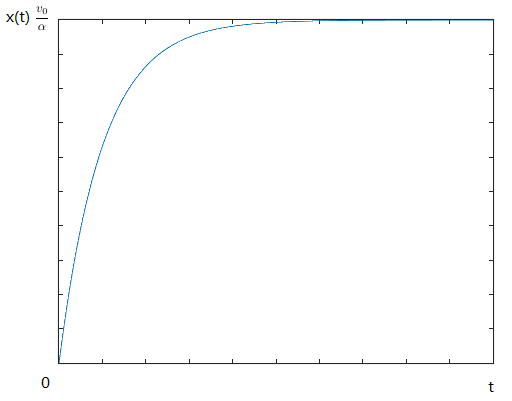
\includegraphics[width=7cm]{x(t).png}
    \caption{$x(t)=\frac{v_0}{\alpha}(1-e^{-\alpha t})$}
    \label{fig-sample}
\end{figure}
\begin{figure}[h!]
    \centering
    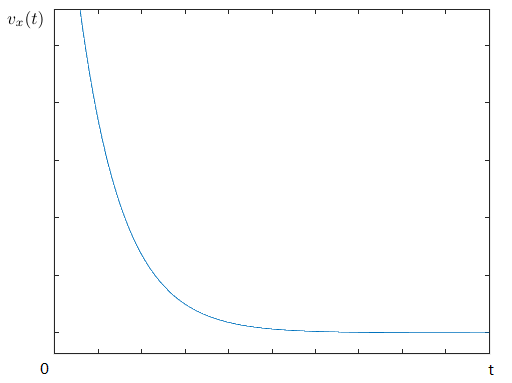
\includegraphics[width=7cm]{v(t).png}
    \caption{$v_x(t)=v_0e^{-\alpha t}$}
    \label{fig-sample}
\end{figure}
\newpage
\begin{figure}[h!]
    \centering
    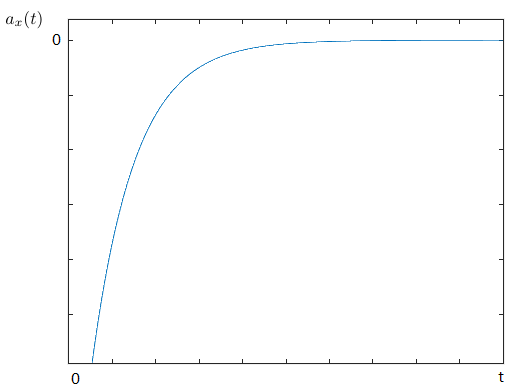
\includegraphics[width=7cm]{a(t).png}
    \caption{$a_x(t)=-\alpha v_0e^{-\alpha t}$}
    \label{fig-sample}
\end{figure}

\item

When we research the movement of an object under air resistance at a relative slow speed, 
the acceleration of the object is $a=-\frac{kSv}{m}$,\\
which is similar to the model when $\alpha =\frac{kS}{m}$
\end{enumerate}

\section*{Problem 9.}
According to chain rule,
$$\frac{dv_x}{d_t}dx=\frac{dx}{dt}dv_x$$\\
Thus,
$$a_xdx=v_xdv_x$$

\section*{Problem 10.}
\begin{enumerate}[(a)]
\item
$$\frac{dx}{dt}=\sqrt{px} \Longrightarrow \frac{dx}{\sqrt{px}}=dt$$
Do integration on each side, 
$$x^{\frac{1}{2}}=\frac{\sqrt{p}t}{2}+C$$
$$x=\left(\frac{\sqrt{p}t}{2}+C\right)^2$$
When $t=0$, $x=0$, so
$$x=\frac{p}{4}t^2$$
$$v_x=\frac{dx}{dt}=\frac{p}{2}t$$
$$a=\frac{dv_x}{dt}=\frac{p}{2}$$
\item
$$s=\frac{1}{2}at^2=\frac{p}{4}t^2 \Longrightarrow t=2\sqrt{\frac{s}{p}}$$
$$\bar{v}=\frac{s}{t}=\frac{\sqrt{ps}}{2}$$
\item
It is a constant x-acceleration motion.

\end{enumerate}

\section*{Problem 11.}
The statement is based on the assertion that space can de divided infinitely, but it is proved to be false in modern science and physics.\\
According to quantum physics, the smallest length is Planck's unit of length, $l_p$, of about $1.616199\times 10^{-35}\ m$.
When the distance between the tortoise and the Achilles is less than $l_p$, in the next immediate of time, the Achilles would outstrip the tortoise.

\section*{Problem 12.}
Set the speed of the fisherman and river $v,\ v_0\ km/h$.\\
Assume that the fisherman spend $t$ hours after he turned around.\\
We will have the equations:
\begin{eqnarray*}
\left\{
\begin{array}{lll}
(t+1)v_0+(t-1)v&=&6\\
(t+1)v_0&=&6\\
\end{array}
\right.\quad\Rightarrow\quad
\left\{
\begin{array}{lll}
t&=&1\\
v_0&=&3\\
\end{array}
\right.
\end{eqnarray*} 
So the spped of the river;s current is 3 $km/h$


\section*{Problem 13.}
According to the conditions,
\begin{align*}
t_1&=\frac{2L}{\sqrt{v^2-c^2}}\\
t_2&=\frac{L}{v+c}+\frac{L}{v-c}=\frac{2vL}{v^2-c^2}\\
t_1-t_2&=2L\left(\frac{1}{\sqrt{v^2-c^2}}-\frac{v}{v^2-c^2}\right)=2L\left(\frac{\sqrt{v^2-c^2}-v}{v^2-c^2}\right)<0
\end{align*}
So Boat 1 will win the race.
\end{document}